\section{Zielsetzung}
\label{sec:Zielsetzung}
Da die technik und Freizeit (z.B. Tauchen oder Fallschirmspringen) ohne die Erforschung und Verwendung von Unterdruck- und Vakuumbereichen nicht vorzustellen
ist, sollen in diesem Versuch die Grundlagen der Vakuumtechnik genauer betrachtet werden.
Genauer soll der Aufbau eines Pumpstandes zur Bestimmung von Evakuierungskurven und Leckratenmessungen
bei einer Drehschieberpumpe und einer Turbomolekularpumpe (im weiteren als TMP bezeichnet) verwendet werden.
Aus diesen Daten sollen dann das effektive Saugvermögen berechnet und gegen die Druckabhängigkeit dargestellt werden.


\section{Theorie:}
\label{sec:Theorie}
\subsection{Grundbegriffe}

Im folgenden werden zunächst einmal die wichtigsten Begriffe der Vakuumphysik näher erläutert:
\paragraph{Vakuum:}
Die Allgemeine Annahme, dass das Vakuum ein vollständig leerer Raum ist, ist nach Definition der
deutschen Industrienorm nicht korrekt.
Ein Vakuum ist dort definiert als "der Zustand eines Gases, wenn in einem Behälter der
Druck des Gases und damit die Teilchenzahldichte niedriger ist als außerhalb oder wenn der Druck
des Gases niedriger ist als 300 mbar, d. h. kleiner als der niedrigste auf der Erdoberfläche
vorkommende Atmosphärendruck."\cite{vakuum}

Das Vakuum kann in einzelne Bereiche unterteilt werden, die abhängig von ihrem Druckbereich und der mittleren
freien Weglänge der in diesem Bereich befindlichen Teilchen ist.
Eine solche Unterteilung ist in Tabelle \ref{tab:Vakuum} zu finden.

\begin{table}
  \centering
  \caption{Druckbereiche mit konventionellem Namen, Teilchendichte und mittlerer freien Weglänge.}
  \label{tab:Vakuum}
  \begin{tabular}{cccc}
    \toprule
    &$p$ in mbar & n in Teilchen/cm$^3$ & $\lambda$ \\
    \midrule
    Umgebungsdruck & 1013 & 2,7\cdot10$^{19}$ & \SI{68}{\nano\meter} \\
    Unterdruck & > 300 & > 10$^{19}$ & < \SI{0.1}{\micro\meter} \\
    Grobvakuum & 300 - 1 & 10$^{19}$ - 10$^{16}$ & 0,1 - 100$\,\mu$m \\
    Feinvakuum & 1 - 10$^{-3}$ & 10$^{16}$ - 10$^{13}$ & 0,1 - 100$\,$mm \\
    Hochvakuum & 10$^{-3}$ - 10$^{-7}$ & 10$^{13}$ - 10$^{9}$ & 10$\,$cm - 1$\,$km \\
    Ultrahochvakuum & 10$^{-7}$ - 10$^{-12}$ & 10$^{9}$ - 10$^{4}$ & 1$\,$km - 10$^5\,$km \\
  \end{tabular}
\end{table}

\paragraph{Druck und Partialdruck:}
"Der Druck ist definiert als der Betrag einer senkrecht und gleichmäßig auf eine Flächeneinheit wirkenden Kraft."\cite{pfeiffer}
\begin{equation}
  p = \frac{F}{A}
\end{equation}
Da ein Gas wie z.B. Luft nicht nur aus einer Teilchensorte besteht und jede Sorte seinen eigenen Anteil zum Gesamtdruck darstellt, werden
die einzelnen entstehenden Drücke als Partialdruck bezeichnet. Eine graphische Darstellung der Druckarten ist in \ref{fig:Druck} zu finden.

\begin{figure}
  \centering
  \begin{subfigure}[b]{0.48\textwidth}
    \centering
    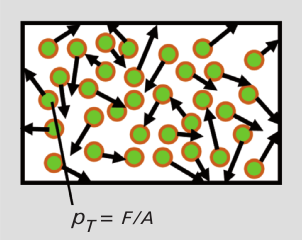
\includegraphics[width=\textwidth]{Druck.png}
  \end{subfigure}
  \begin{subfigure}[b]{0.49\textwidth}
    \centering
    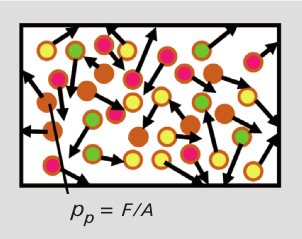
\includegraphics[width=\textwidth]{Partialdruck.png}
  \end{subfigure}
  \caption{Graphische Darstellung von Druck und Partialdruck durch Impulse von Teilchen \cite{pfeiffer}.}
  \label{fig:Druck}
\end{figure}

\paragraph{Mittlere freie Weglänge:}
Die mittlere freie Weglänge $\lambda$ ist definiert als die durchschnittliche Weglänge, die
ein Teilchen zurücklegt, bis es zu einem Stoß mit einem anderen Teilchen kommt.
\begin{equation}
  \lambda = \frac{1}{n\cdot\sigma}
  \label{eqn:Weglaenge}
\end{equation}
\begin{equation*}
  n:\text{Teilchenzahldichte, } \sigma:\text{Wirkungsquerschnitt}
\end{equation*}
Bei Verwendung eines idealen Gases, bei dem sich die Teilchen nach der Maxwellschen Geschwindigkeitsverteilung
bewegen, gilt
\begin{equation}
  \lambda = \frac{k_\text{B}T}{\sqrt{2}\pi p d^2} \\
\end{equation}
\begin{equation*}
  k_\text{B}:\text{Boltzmann-Konstante }, T:\text{Temperatur}, d:\text{Durchmesser d. Moleküls }, p:\text{Druck}
\end{equation*}
\paragraph{Ideales Gas:}
Das ideale Gas ist ein Modell aus der Thermodynamik um gas möglichst einfach beschreiben zu
können. Dabei wird davon ausgegangen, das die Gasteilchen nur untereinander oder mit den Wänden
(indem sich das entsprechende gas befindet) elastisch stoßen. Daraus lässt sich die ideale Gasgleichung
\begin{equation}
  p \cdot V = N \;k_\text{B}\;T \\
  \label{eqn:ideal}
\end{equation}
\begin{equation*}
  p:\text{Druck }, V:\text{Volumen d. Gefäßes }, N:\text{Teilchenzahl}
\end{equation*}
folgern.

Von besonderer Bedeutung ist im Verlauf dieses Experimentes das Gesetz von Boyle-Mariotte, welches bewegt,
dass bei konstanter Temperatur der Zusammenhang
\begin{equation}
  p \sim V^{-1}
\end{equation}
gilt.

\paragraph{Stömungsarten:}
Bei der Unterscheidung von verschiedenen Strömungsarten ist die Knudson-Zahl $K_n$ von großer
Bedeutung. Diese ist definiert als die mittlere freie Weglänge pro charakteristischer Länge des
durchströmten Mediums.
\begin{equation}
  K_N = \frac{\lambda}{l}
  \label{eqn:Knudsen}
\end{equation}
Für eine Knudsen-Zahl zwischen 0,01 und 0.5 wird der begriff Knudsen-Strömung verwendet. Diese
Knudsen-Strömung taucht besonders im Bereich des Feinvakuums auf, diese tritt oft in technischen Anwendungen
auf.
Bei einer Knudsen-zahl von $K_n < 0,01$ wird von einer Kontinuumsströmung gesprochen, die vorallem im
Grobvakuum auftritt. Im weiteren beschräftigen wir uns mit der laminaren- und der turbulenten Strömung.
Gilt $K_n > 0,5$, so ist die mittlere freie Weglänge wesentlich größer als die Abmessung des Strömungskanals
und es lassen sich kann noch Wechselwirkungen mit anderen Gasteilchen feststellen. Es kommt zur molekularen
Strömung, diese ist vorallem im Bereich des Hoch- und Ultrahochvakuums aufzufinden.

\subsection{Vakuumtechnik:}
Bei der Unterscheidung von verschiedenen Typen von Vakuumpumpen kommt es auf die verschiedenen Arten der
Wechselwirkung zwischen Gasteilchen und Wänden an.

\paragraph{Sorption:}
Als Sorption bezeichnet man die aufnahme eines Teilchens durch Ab- oder Adsorption.

\paragraph{Absorption:}
Dies ist die Aufnahme eines Atoms, Moleküls oder Ions, welches von einer anderen Phase vollständig
aufgenommen wird.

\paragraph{Adsorption:}
Anders als bei der Absorption, wird dat Atom, Molekül oder Ion hier nur auf der Oberfläche der anderen Phase
festgehalten und nicht komplett aufgenommen.

\paragraph{Desoption:}
Dies ist die Umkehrung der Sorption, also die Abgabe eines Atoms, Moleküls oder Ions.

 \paragraph{Diffusion:}
 Dies ist der Ausgleich bzw. Konzentrationsausgleich zwischen zwei verschieden konzentrierter Bereiche
 aufgrund von brownscher Molekularbewegung. In der Vakuumsphysik tritt dies auf, wenn es wärend des Anlegen eines
 Vakuums zu einem Gasdruckabfalls im Rezipienten kommt.

 Da es auf der Erde kein natürliches Vakuum gibt, ist es unverzichtbar auf Vakuumpumpen zurückzugreifen. Hier werden
 2 Arten von Vakuumpumpen betrachtet:

 \paragraph{Drehschieberpumpe:}
 Die Drehschieberpumpe gehört zur Kategorie der Gastransferpumpen und besteht aus einem Gehäuse (auch Stator genannt), einem
 exzentisch eingebautem Rotor und einem im Rotor eingebautem Schieber, welcher mit seiner Feder an das Gehäuse gedrückt wird.
 Ein- und Ausgang des Gehäuses sind durch Ventile gesichert. Dieser Aufbau ist in Abbildung \ref{fig:DSP} zu finden.
 Der Schieber teilt den Arbeitsraum in Druck- und Saugbereich ein. Fährt der schieber an dem Einlassventil vorbei, so strömt
 das gas in das "neu" enstandene Volumen. Nachdem der Einlass wieder geschlossen ist, wird das Gas zwischen den zwei Scheiben komprimiert.
 Ist der Druck groß genug, so öffnet sich das Auslassventil (Federventil) und das Gas strömt heraus. Während dieses Vorganges
 befindet sich immer etwas Öl im Arbeitsraum um den Schieber zu schmieren und den Raum abzudichten.

 Diese Art von Vakuumpumpe wird im bis zu einem Feinvakuum als Hauptpumpe verwendet. Bei einem Hochvakuum und weitern Druckbereichen wird
 ein solches Gerät als Vorpumpe verwendet, z.B. vor einer TMP.

 \begin{figure}
   \centering
   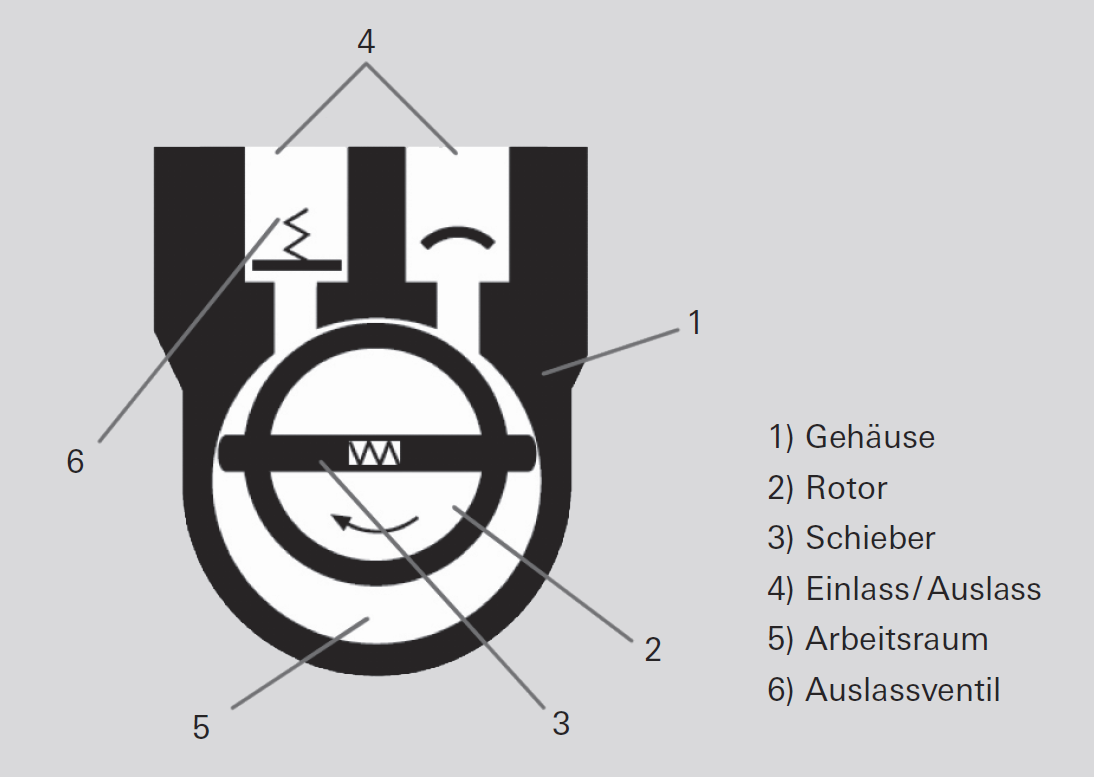
\includegraphics[width=0.5\textwidth]{Drehschieberpumpe.png}
   \caption{Schematische Darstellung einer Drehschieberpumpe \cite{DSP}}
   \label{fig:DSP}
 \end{figure}

 \paragraph{Turbomolekularpumpe:}
 Diese von Willi Becker verbesserte Art der Molekularpumpe besteht aus einer mehrstufigen Anordnung von Statoren und Rotoren. Dabei sollen die
 Rotoren den Gasteilchen einen zusätzlichen Impuls geben der sie dazu bringt aus die Statoren zu treffen und abtransportiert zu werden. Dafür
 muss im Rezipienten selbst eine molekulare Strömung vorliegen. Die freie mittlere Weglänge muss zudem größer sein als der Abstand der Rotorblätter.
 Daher muss das Vakuum im Rezipienten schon vor dem einschalten der TMP bei ca. 10$^{-1}\,$mbar liegen. Ansonsten würden die Teilchen zwischen
 den Statoren und Rotoren stoßen und somit wieder auf in den rezipienten gelangen, somit würde man kein höheres Vakuum erschaffen können.
\begin{figure}
  \centering
  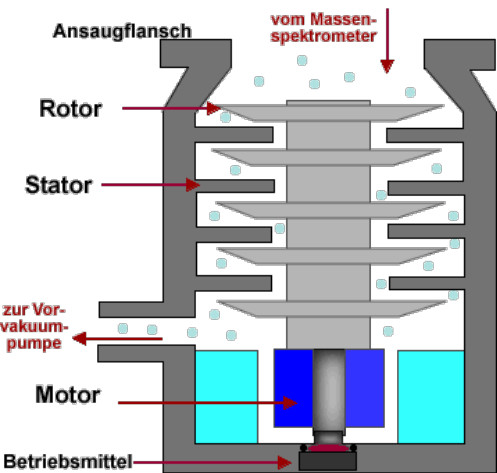
\includegraphics[width=0.5\textwidth]{TMP.pdf}
  \caption{Schematische Darstellung einer Turbomolekularpumpe \cite{TMP}.}
  \label{fig:TMP}
\end{figure}
\FloatBarrier

 \paragraph{Saugvermögen:}
 Zur Bestimmung des Saugvermögens $S$ (geförderter Volumenstrom) müssen folgende theoretische Annahmen getroffen werden \cite{anleitung}:
 \begin{enumerate}
   \item Es gilt während der gesamten Messung: $V = const$
   \item Das verwendete Gas kann als ideales Gas angenommen werden
   \item Die messungen werden bei $T = const$ getätigt
   \item Das Gas ist zu jedem Zeitpunkt im thermischen Gleichgewicht
   \item Lecks und Effekte der Desorption sind zu vernachlässigen
   \item Das Saugvermögen $S$ ist konstant und unabhängig vom Druck
 \end{enumerate}
Wird die ideale Gasgleichung nach der Zeit abgeleitet und eine einfache Pumpe (z.B.Drehschieberpumpe) verwendet, damit $\dot{V} = S$ gilt,
so folgt die Gleichung
\begin{equation}
  \dot{p}V = -pS.
\end{equation}
Dabei wurde die Zeit als konstant angenommen.
Die so entstandene Differentialgleichung lässt sich durch den Exponentialansatz
\begin{equation}
  p(t) = p_0 \text{e}^{-\frac{t}{\tau}}
\end{equation}
lösen. Dabei ist $p_0$ ein gegebener Anfangsdruck. Durch einsetzen ergibt sich
\begin{equation}
  \tau = \frac{V}{S}
\end{equation}
Wird nun ein endlicher Enddruck $p_\text{E}$ berücksichtigt, so folgt die Gleichung
\begin{equation}
  p(t) = (p_0 - p_\text{E})\text{e}^{-\frac{tS}{V}}+p_\text{E}
  \label{eqn:druck}
\end{equation}
Der Einsatz eine Enddrucks folgt aus Effekten wie der Desorption, sowie reale und virtueller Lecks. Durch diee Funktionsweise einer Pumpe kann nun ein
endlicher Enddruck erreicht werden, da Effekte wie Rückstrahlung, Totvolumen sowie endliches Kompressionsvermögen vorliegen können.

\paragraph{Leckrate:}
Um zu ermitteln wieviel Gas pro Zeit aus dem Aufbau geleckt ist, wird die Leckrate $Q$ durch
\begin{equation}
  S  = \frac{Q}{P_\text{G}} \text{ mit } Q = V\,\frac{dp}{dt}
\end{equation}
 defiiniert. Daraus folgt das Saugvermögen
 \begin{equation}
   S = \frac{V}{p_\text{G}}\frac{dp}{dt}.
   \label{eqn:Saug}
 \end{equation}

 \paragraph{Leitwerte:}
 Durch verscshiedene Phänomene wie Strömungswiderstände der Verbindungsstücke wird nie das vom Hersteller versprochene Saugvermögen $S_0$ erreicht.
 Daher wird ein effektives Saugvermögen oder "Nennsaugvermögen" von
 \begin{equation}
   \frac{1}{S_\text{eff}} = \frac{1}{S_0} + \frac{1}{L}
   \label{eqn:effSaug}
 \end{equation}
 erwartet. Dabei ist $L$ der Leitwert, welcher den reziproken Strömunswiderstand darstellt.

 \paragraph{Leck:}
 Als ein Leck wird eine undichte Stelle innerhalb eines Systems bezeichnet, von dem aus Teilchen oder Energie aus dem System
 entweicht odder eindringt.
 In der Vakuummphysik wird zwischen realen und virtuellen Leks unterschieden. Reale Lecks sind physische Löcher bzw. Fehlstellen
 im Aufbau, wohingegen virtuelle Lecks durch Desorption oder Diffusion entstehen und damit keine Fehlstellen darstellen.
 Trotzdem verfälschen diese Effekte ie Messwerte, daher werden durch Ausheizen (erhitzen des Rezipienten) und Fluten (kurzzeitiges
 befüllen mit Stickstoff) die Desorptionsraten so weit es geht gesenkt.

 Zur Messung des Drucks während der Messreihen werden 2 verschiedene Vakuummeter verwendet, dabei hat jedes seinen eigenen Anwendungsbereich:

 \paragraph{Pirani-Messgerät:}
 Für hohe Druckbereiche ($p < \SI{1000}{\milli\bar}$) wird ein Pirani-Messgerät verwendet. Dieses bestimmt den Druck des Gases über die Wärmeleitfähigkeit, welche
 bei kleinem Gasdruck immer kleiner wird und die Temperatur des im Messgerät befestigten Glühdrahts steigt. Dieser Anstieg an Temperatur verursacht einen Widerstand,
 welcher gemessen werden kann. verwendet man dieses Messgerät in einem zu hohen Druckbereich, so wird die Wärmleitung von der Konvektion überdeckt, bei einem zu kleinen
 Bereich von der Wärmestrahlung und der eigentliche zu messende Effekt (Wärmeleitung) tritt in den Hintergrund. Somit sind die Messungen unbrauchbar.

\paragraph{Glüh- und Kaltkathoden Vakuummeter:}
Bei einem Glühkathoden Vakuummeter werden die Elektronen durch thermische Elektronenemission von der Kathode gelöst und die Gasteilchen durch Stöße ionisiert. Die
Anode ist zylindrisch und gitterförmig angeordnet, in ihrer Mitte befindet sich ein als Auffänger dienender Draht, welcher die Ionen aufsammelt. Dieser resultierende
Ionisationsstrom ist ein Maß für den Druck.
Die Funktionsweise des Kaltkathoden Vakuummeters ist nahezu analog zu dem des Glühkathoden Vakuummeters, nur werden die Elektronen dort nicht durch die thermische Elektronenemission,
sondern durch ein starkes äußeres elektrisches Feld aus der Kathode herausgelöst.
